\documentclass[tikz,border=2pt]{standalone}
\usepackage{amsmath}
\usetikzlibrary{arrows.meta}
\begin{document}
% Sample path of a FIFO single-server queue with x = (1,1,3,1,4), s = (3,2,1,2,1):
% A = (1,2,5,6,10), service starts (1,4,6,7,10), D = (4,6,7,9,11), W = (0,2,1,1,0).
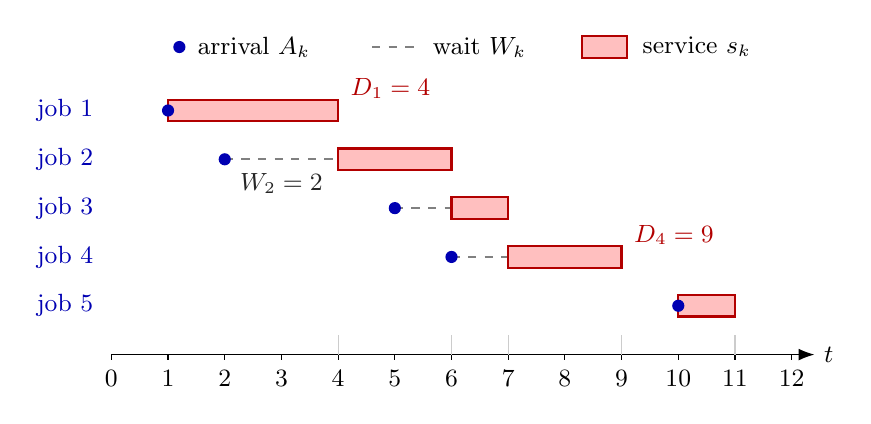
\begin{tikzpicture}[font=\small, >={Latex[length=2mm]}, x=0.72cm, y=0.62cm]
  % time axis
  \draw[->] (0,-6) -- (12.4,-6) node[right] {$t$};
  \foreach \t in {0,...,12} {\draw (\t,-6) -- (\t,-6.12) node[below] {$\t$};}
  % light grid at departure times
  \foreach \d in {4,6,7,9,11} {\draw[gray!40, thin] (\d,-5.6) -- (\d,-6);}
  % jobs: arrival, start, departure, row
  \foreach \k/\a/\s/\d in {1/1/1/4, 2/2/4/6, 3/5/6/7, 4/6/7/9, 5/10/10/11} {
    \node[blue!70!black, anchor=east] at (-0.15,-\k) {job $\k$};
    \draw[gray, thick, dashed] (\a,-\k) -- (\s,-\k);
    \fill[red!25] (\s,-\k-0.22) rectangle (\d,-\k+0.22);
    \draw[red!70!black, thick] (\s,-\k-0.22) rectangle (\d,-\k+0.22);
    \fill[blue!70!black] (\a,-\k) circle (2.2pt);
  }
  % annotations
  \node[gray!30!black, anchor=north] at (3,-2-0.1) {$W_2=2$};
  \node[red!70!black, anchor=west] at (4.05,-0.55) {$D_1=4$};
  \node[red!70!black, anchor=west] at (9.05,-3.55) {$D_4=9$};
  % legend
  \fill[blue!70!black] (1.2,0.3) circle (2.2pt);
  \node[anchor=west] at (1.35,0.3) {arrival $A_k$};
  \draw[gray, thick, dashed] (4.6,0.3) -- (5.4,0.3);
  \node[anchor=west] at (5.5,0.3) {wait $W_k$};
  \fill[red!25] (8.3,0.08) rectangle (9.1,0.52);
  \draw[red!70!black, thick] (8.3,0.08) rectangle (9.1,0.52);
  \node[anchor=west] at (9.2,0.3) {service $s_k$};
\end{tikzpicture}
\end{document}
